
% Begin with describing virtual circuit switching
\begin{section}{Introduction: Packet Queueing in Switches}


\end{section}


\begin{section}{Challenges}

\end{section}

\begin{section}{Experiment}


\end{section}

\begin{section}{Variables of the Experiment}

    \begin{subsection}{Packet Generation Probability $p$}
        Each input port generates a packet in a time slot with a Bernoulli$(p)$ distribution.
    \end{subsection}

    \begin{subsection}{Buffersize $B$}
    Each input and output can hold upto $B$ packets
    \end{subsection}

\end{section}

\begin{section}{iSLIP Algorithm}
    \begin{subsection}{Algorithm}
        
    \end{subsection}

    \begin{subsection}{Time Complexity}
        
    \end{subsection}

    \begin{subsection}{Salient Features}

    \end{subsection}

\end{section}


\begin{section}{Results}

    \begin{figure}[htbp]
        \centering
        % First figure (fig1a)
        \begin{subfigure}[b]{0.45\textwidth}
            \centering
            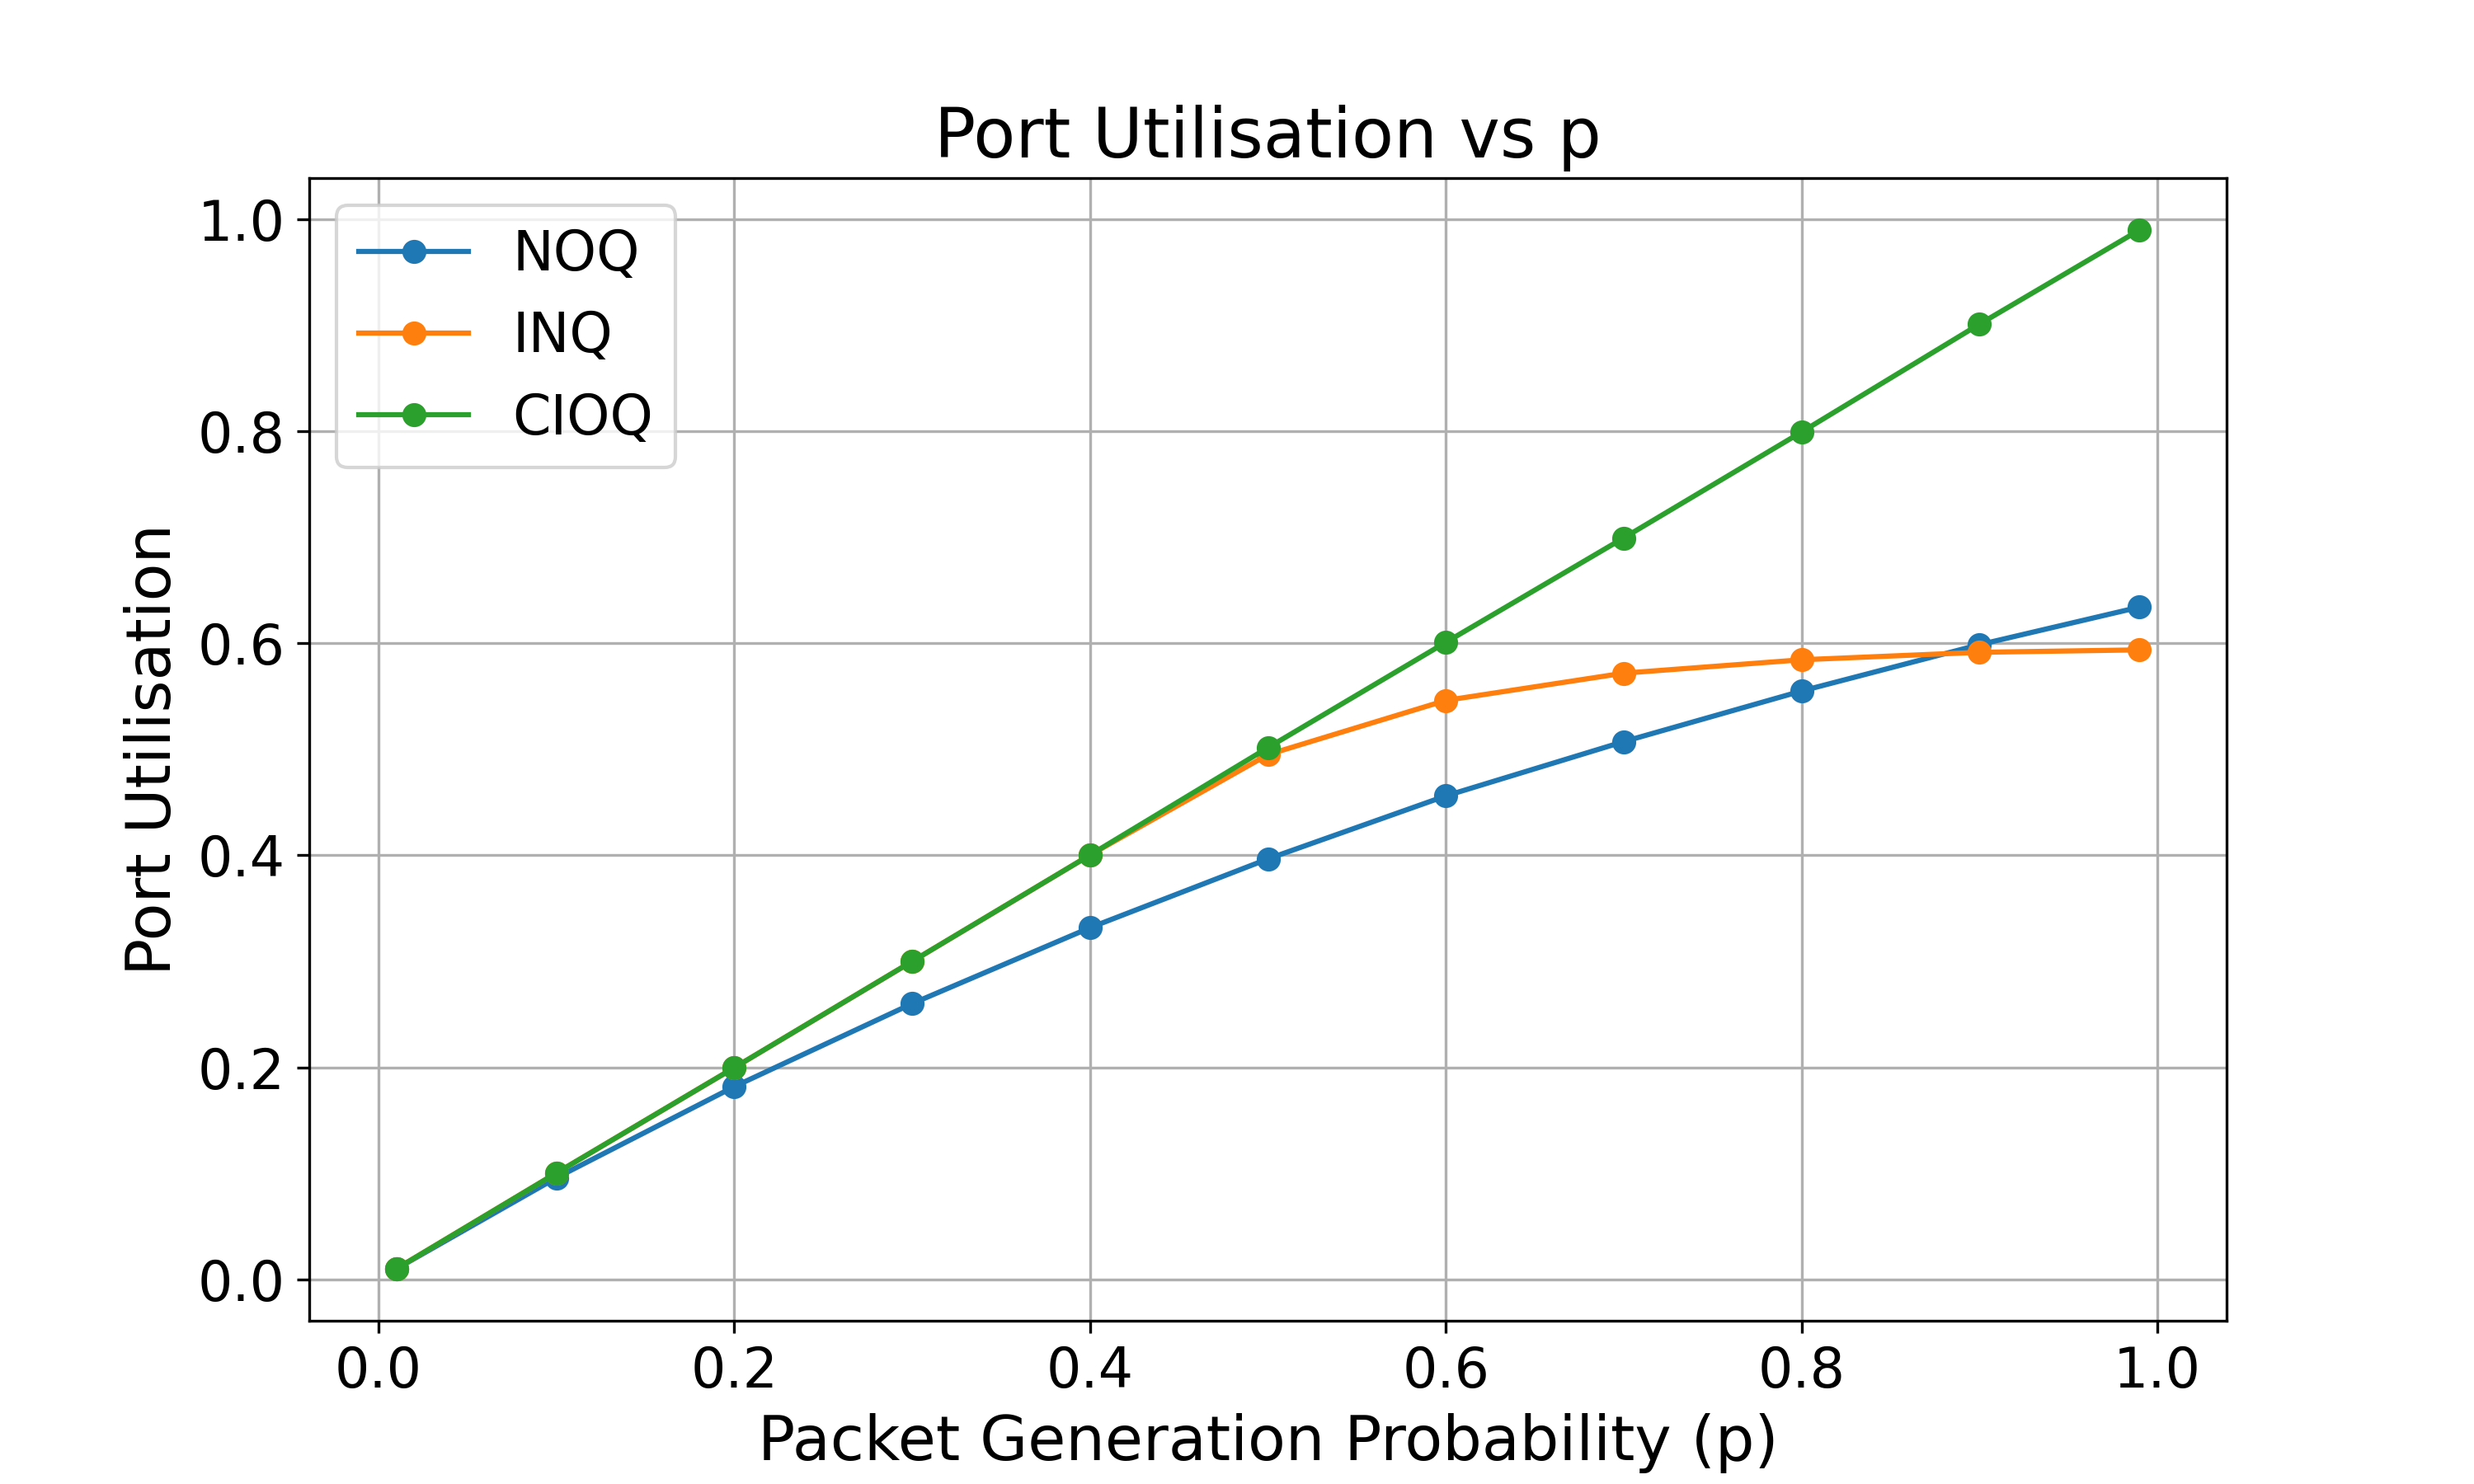
\includegraphics[width=\textwidth]{figures/fig1/fig1a.png}
            \caption{Utilisation}
            \label{fig:utilisation}
        \end{subfigure}
        \hfill
        % Second figure (figures/fig1/fig1b)
        \begin{subfigure}[b]{0.45\textwidth}
            \centering
            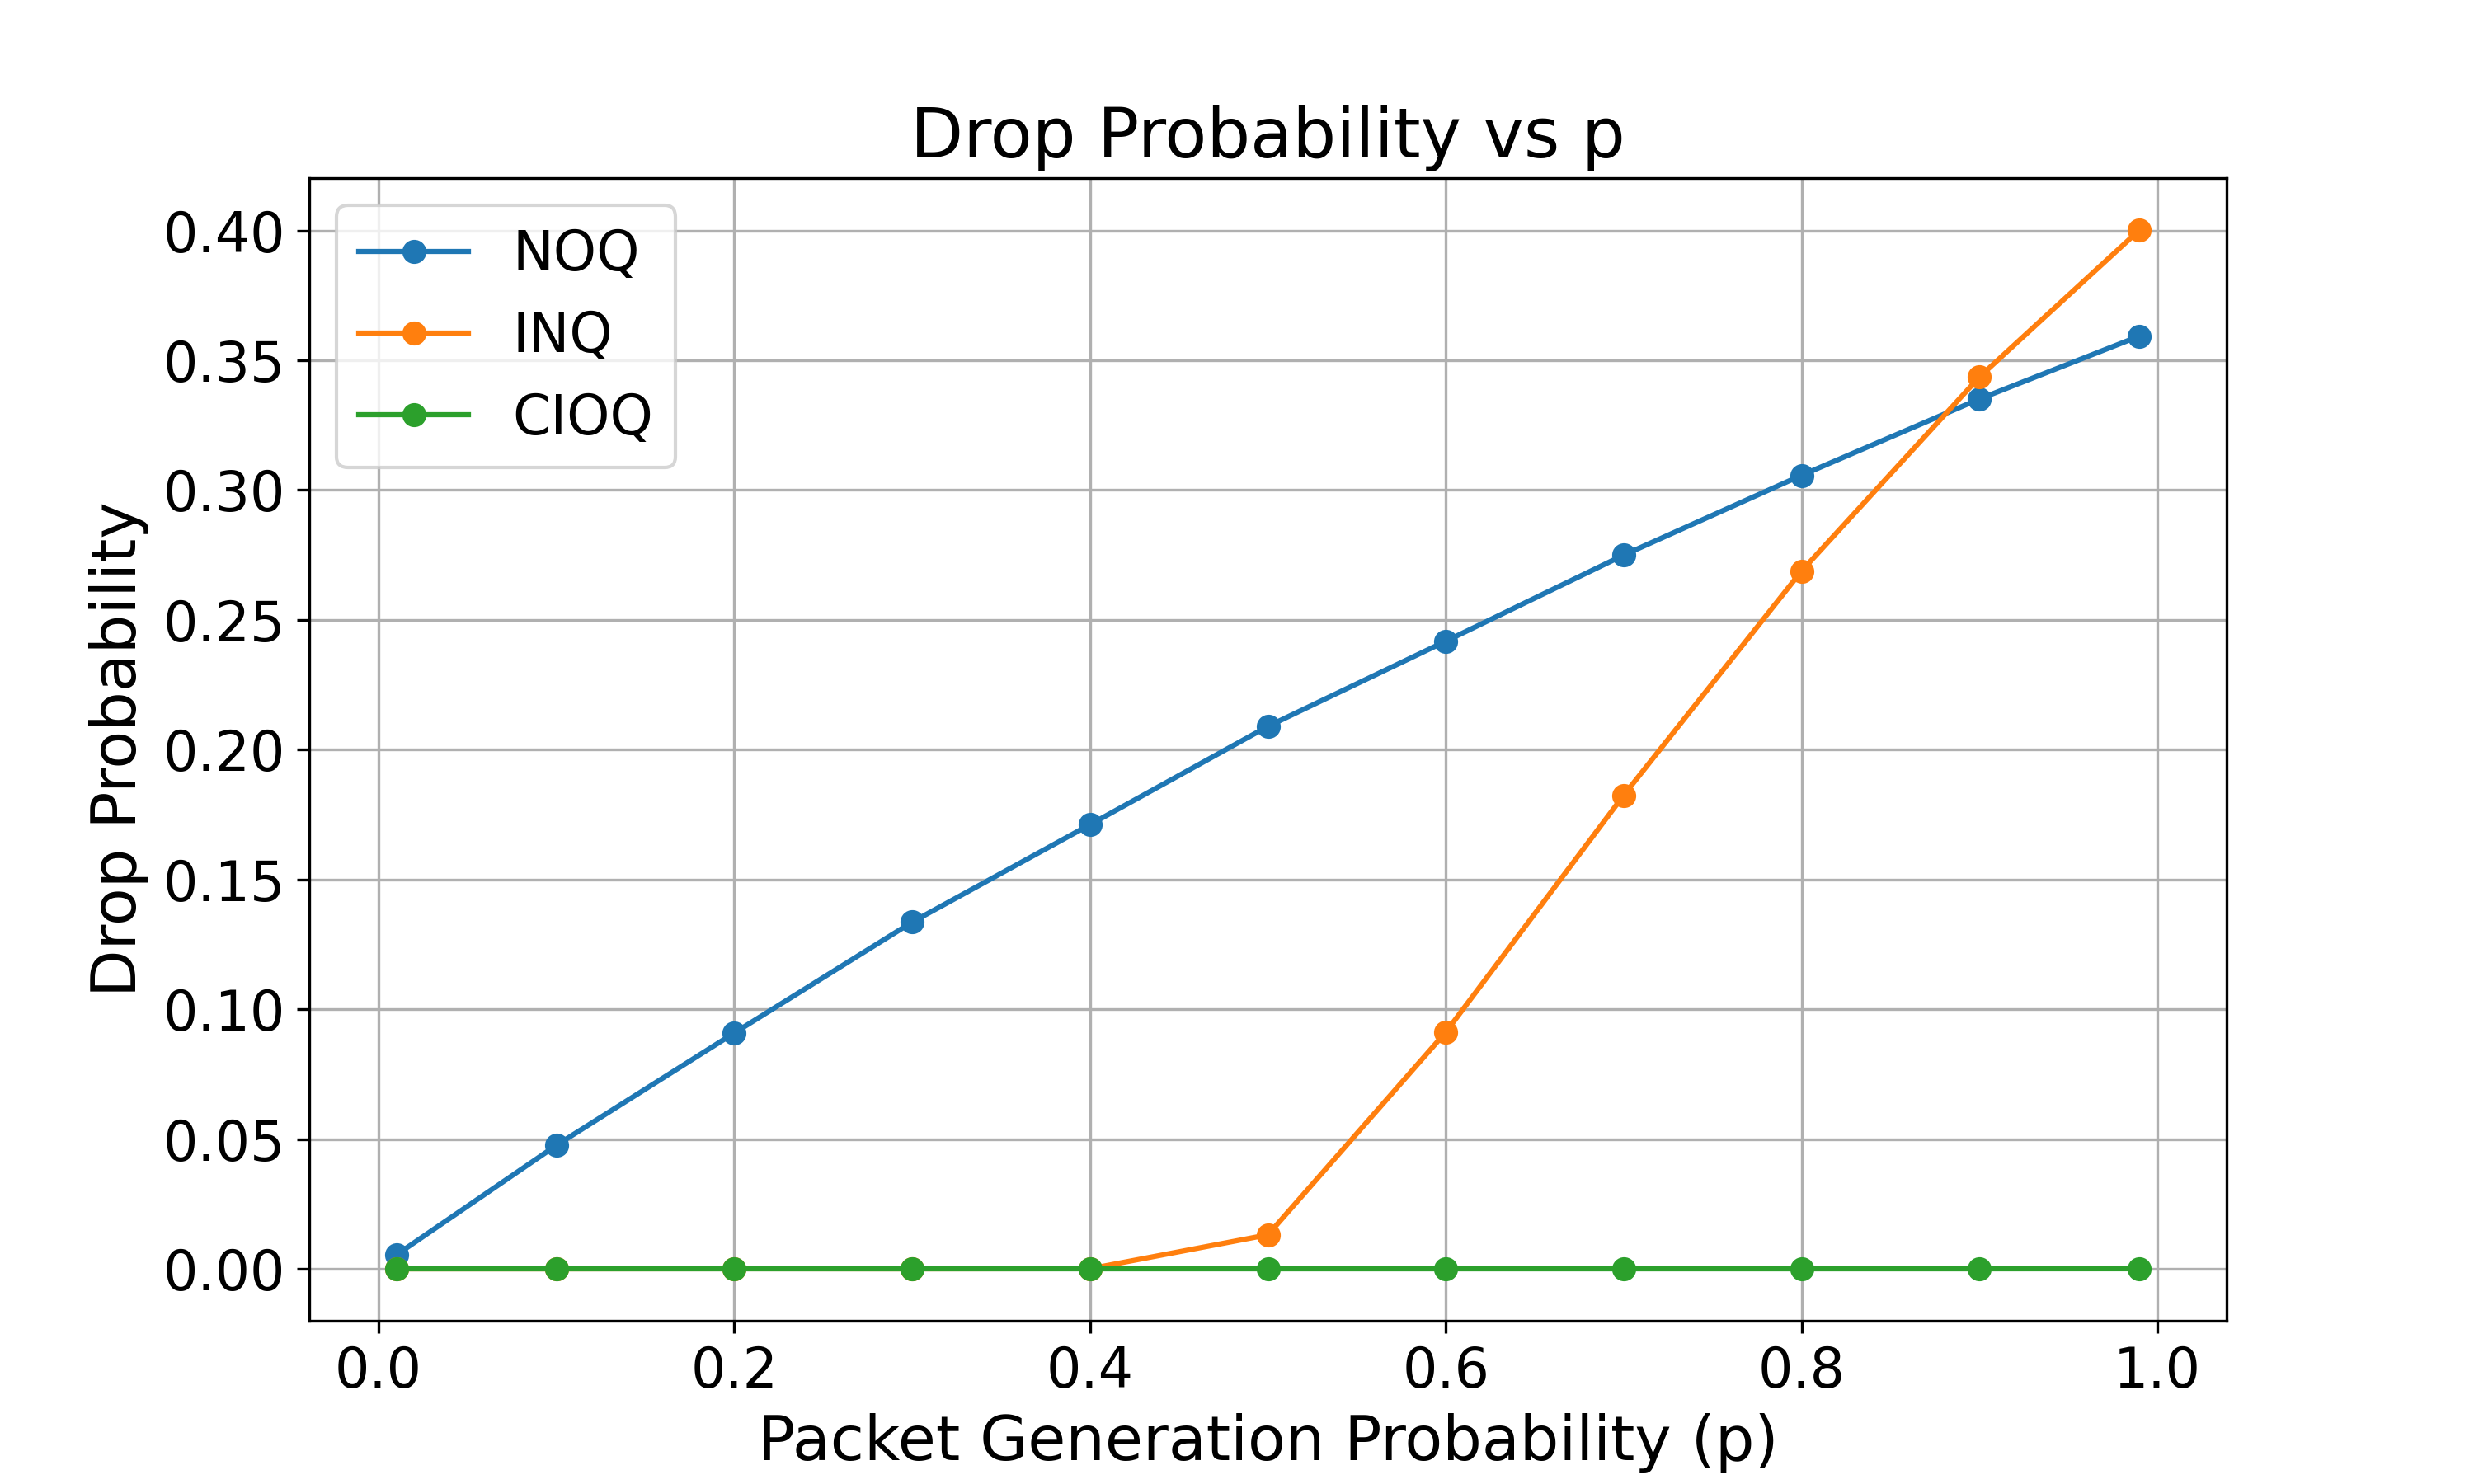
\includegraphics[width=\textwidth]{figures/fig1/fig1b.png}
            \caption{Drop Probability}
            \label{fig:drop_prob}
        \end{subfigure}
        \hfill
        % Third figure (figures/fig1/fig1c)
        \begin{subfigure}[b]{0.45\textwidth}
            \centering
            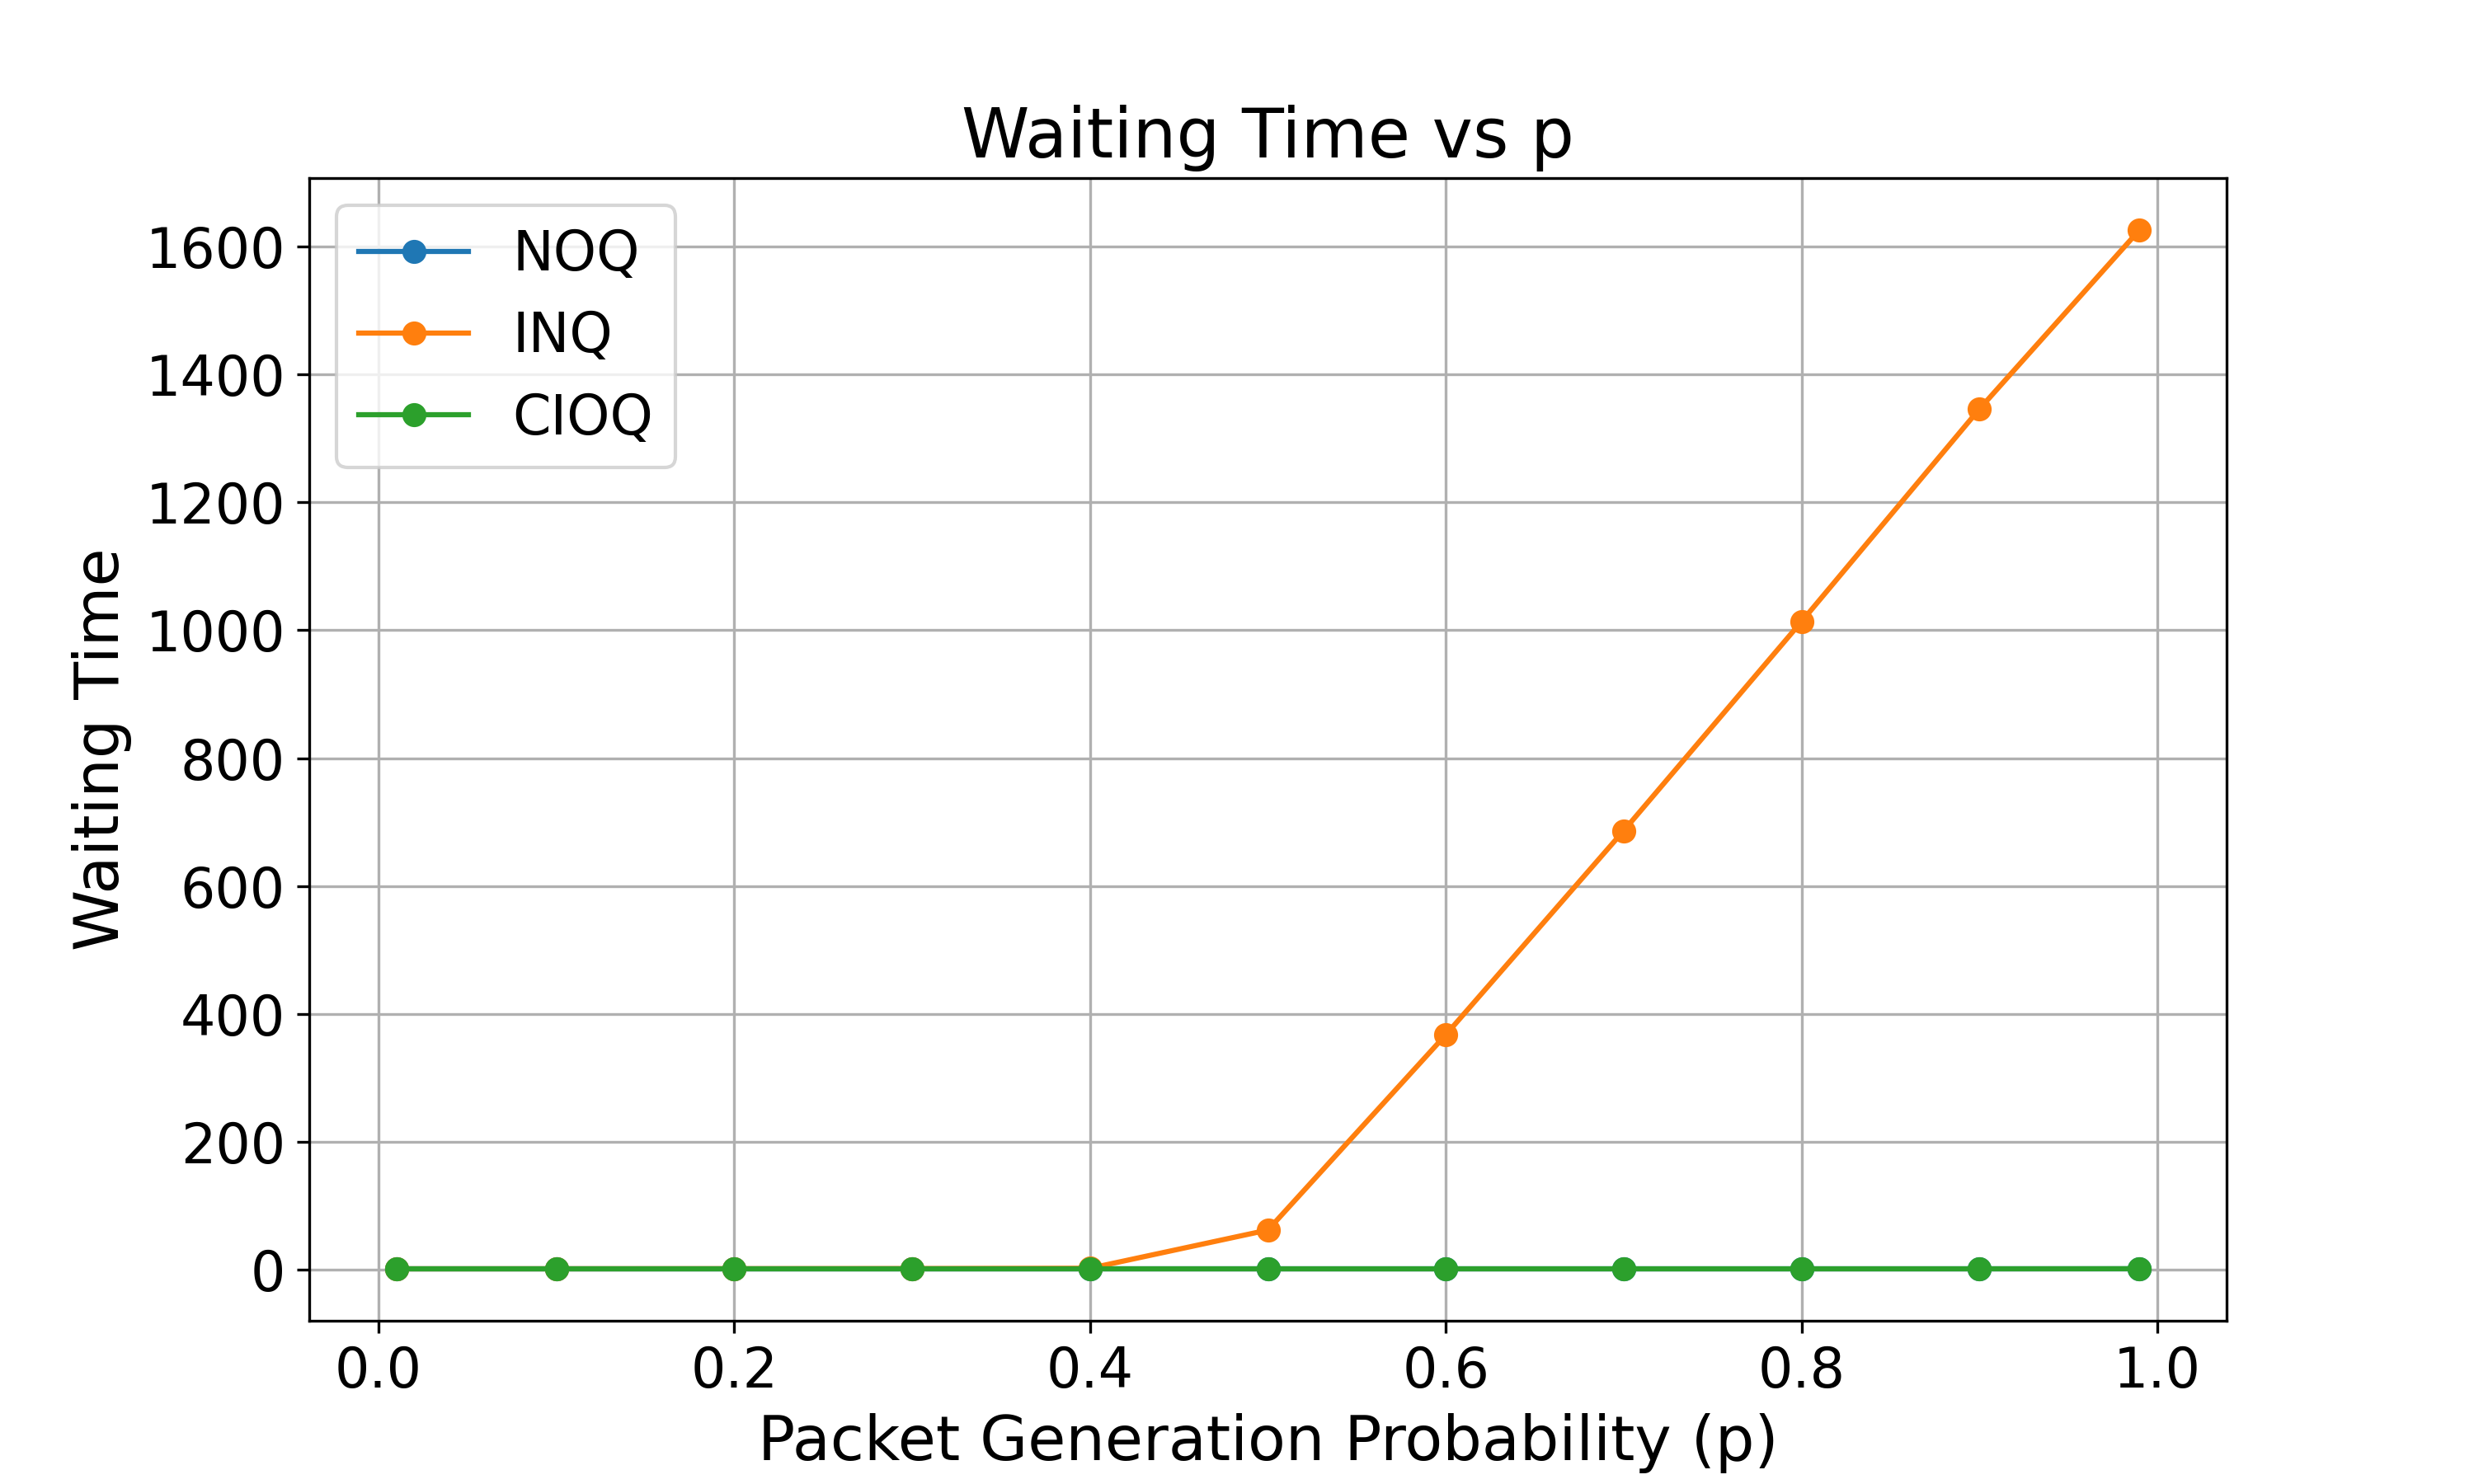
\includegraphics[width=\textwidth]{figures/fig1/fig1c.png}
            \caption{Wait Time}
            \label{fig:wait_time}
        \end{subfigure}
        
        \caption{Comparing the different Queueing algorithms}
        \label{fig:combined}
    \end{figure}

    The above figure compares the link utilisation, drop probability and waiting time for the different algorithms with default parameters. For CIOQ, $K=4$ and $L=6$ was chosen. 
    \begin{subsection}{Utilisation}
        From the figure we see that iSLIP algorithm has the best utilisation and increasing linearly with the increase in probability. As derived in class, we see that NOQ has a saturation utilisation of $64\%$ while INQ can only have a maximum utilisation of $58.6\%$.
        One important insight from this is that although NOQ outperforms INQ, at lower loads, the INQ gives a much better utilisation than NOQ. 
    \end{subsection}

    \begin{subsection}{Drop Probability}
        CIOQ with iSLIP algorithm has as a consistent nearly 0 drop probability, whereas NOQ and IOQ have drop probabilities reaching to upto 40\% for $p=1$. Again, here INQ outperforms NOQ under low loads, but becomes worse under higher loads.
    \end{subsection}

    \begin{subsection}{Waiting Time}
    The waiting time for NOQ and CIOQ is consistently 1 time slot. But for INQ, the wait time increase approximately linearly after $p=0.5$, and reached a maximum of 1600 time slots. Thus, considering waiting time as the metric, NOQ and CIOQ are preferred.
    \end{subsection}
    

\end{section}

\begin{section}{Conclusion}

\end{section}
